We will now consider sheaf cohomology on the \'etale site. 

\begin{theorem}
  A presheaf $\Sh{F}$ on $\text{\'Et}/X$ is a sheaf if and only if $\Sh{F}$ satisfies the sheaf condition for Zariski open coverings and for \'etale coverings consisting of a single map $V \to U$, where $V$ and $U$ are affine.
\end{theorem}
\begin{proof}
  See \cite{milneLEC}, .
\end{proof}
\begin{corollary}
  Every presheaf represented by an $X$-scheme $U \to \Hom_X(U,Z)$ is a sheaf. 
\end{corollary}
\begin{proof}
  It is obviously a sheaf for the Zariski topology. (...)
\end{proof}

\begin{definition}[Constant sheaves]
  Let $X$ be a quasi-compact scheme. 
\end{definition}

\begin{definition}[Locally constant sheaves]
  A sheaf $F$ on $X$ is locally constant if there is an \'etale covering $\{U_i\}$ of $X$ such that $F|_{U_i}$ is a constant sheaf for each $U_i$.
\end{definition}

\begin{proposition}
  Let $X$ be a connected scheme and $x$ a geometric point of $X$. The functor $F \to F_{\overline{x}}$ induces an equivalence between the category of locally constant sheaves of sets with finite stalks on $X$ and the category of finite $\pi_1^{\acute{e}t}(X,\overline{x})$-sets.
\end{proposition}
\begin{proof}
  
\end{proof}

\subsection{Galois theory for \'etale covers}
\begin{definition}[The fiber functor $F_x$]
  Let $x: \Spec(\Omega) \to X$ be a geometric point, where $\Omega$ is an algebraically field. The fiber functor at $x$ associates to each \'etale cover $f: Y \to X$ the underlying set of $\Spec(\Omega) \times_X Y$.
\end{definition}

\begin{definition}[Galois covers]
  A connected finite \'etale cover $Y \to X$ is \textit{Galois} if its group of $X$-automorphism acts transitively on geometric fibers.
\end{definition}

\begin{theorem}
  If $X$ is an irreducible topological space and $\Sh{F}$ is a constant sheaf, then $H^r(X, \Sh{F})$ for all $r>0$.
\end{theorem}
\begin{proof}
  Since any open set $U \subseteq X$ is connected, $\Sh{F}(U) = G$ if $\Sh{F}$ is the constant sheaf defined by the group $G$ and $U$ is nonempty. This means that $\Sh{F}$ is flasque, hence $H^r(X, \Sh{F})$ for all $r>0$.
\end{proof}
It follows that constant sheaves on varieties have no higher cohomology. The reason ist that there are not enough open sets in the Zariski topology. This was the reason for defining the \'etale topology. We will now see how the \'etale topology yields good cohomological results

As we have seen, sheaves relate the local and global information one has on a given topological space $X$. In a sense sheaf cohomology measures how much more information we gain when we go from global to local. For example, consider the sheaf of local sections of the covering space $\pi : X \to S^1$.

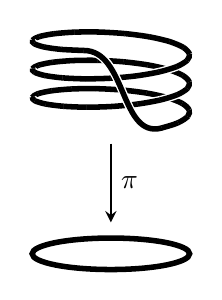
\begin{tikzpicture}[declare function={f(\x)=0.2*sin(\x)+\x/1000;},
  rubout/.style={/utils/exec=\tikzset{rubout/.cd,#1},
  decoration={show path construction,
       curveto code={
        \draw [white,line width=\pgfkeysvalueof{/tikz/rubout/line width}+2*\pgfkeysvalueof{/tikz/rubout/halo}] 
         (\tikzinputsegmentfirst) .. controls
         (\tikzinputsegmentsupporta) and (\tikzinputsegmentsupportb)  ..(\tikzinputsegmentlast); 
        \draw [line width=\pgfkeysvalueof{/tikz/rubout/line width},shorten <=-0.1pt,shorten >=-0.1pt] (\tikzinputsegmentfirst) .. controls
         (\tikzinputsegmentsupporta) and (\tikzinputsegmentsupportb) ..(\tikzinputsegmentlast);  
       }}},rubout/.cd,line width/.initial=2pt,halo/.initial=0.5pt]
  \draw[rubout={line width=2pt,halo=0.5pt},decorate] 
    plot[variable=\x,domain=-50:970,samples=55,smooth] ({cos(\x)},{f(\x)}) to[out=0,in=195] cycle;
  \draw[line width=2pt] (0,-2) arc(-90:270:1cm and 0.2cm);
  \draw[thick,-stealth]  (0,-0.4) -- (0,-1.4) node[midway,right]{$\pi$};
 \end{tikzpicture} 

There is no global section $s: S^1 \to X$ but locally, the set of sections $\{s: U \to \pi^{-1}(U) | \pi \circ s = id$ is a set with three elements.

Let $X$ be a topological space. A theorem of algebraic topology says that for any abelian group $A$, the cohomology group $H^1(X,A)$ with coefficients in $A$ is isomorphic to the abelianisation of the fundamental group $\pi_1(X)$